\documentclass[a4paper,11pt]{article}
\pdfoutput=1 % if your are submitting a pdflatex (i.e. if you have
             % images in pdf, png or jpg format)

\usepackage{jinstpub} % for details on the use of the package, please
                     % see the JINST-author-manual

\usepackage{xcolor,soul,framed} %,caption

%Mathabx do not work on ScribTex => Removed
%\usepackage{mathabx}

\usepackage{mdwmath}
\usepackage{mdwtab}
\usepackage{eqparbox}
\usepackage{url}
\usepackage{dblfloatfix}    % To enable figures at the bottom of page
\usepackage{kantlipsum}     % for random text
\usepackage{hyperref}
\usepackage[export]{adjustbox}

\begin{document}
%\bstctlcite{IEEEexample:BSTcontrol}
    \title{Optimal Planar X-ray Imaging Soft Tissue Segmentation Using a Photon Counting Detector}
    
\author[a,1]{Jericho~O'Connell,\note{Corresponding author.}}
\author[b]{Kris~Iniewski}% <-this % stops a space
\author[a]{Magdalena~Bazalova-Carter}

\emailAdd{jerichoo@uvic.ca}

\affiliation[a]{University of Victoria,\\3800 Finnerty Rd, Victoria, BC, Canada}
\affiliation[b]{Redlen Technologies,\\123 - 1763 Sean Heights
Saanichton, BC, Canada}

\abstract{
A rigorous method for automated soft tissue segmentation using planar kilovoltage (kV) imaging, a photon counting detector (PCD), and a convolutional neural network is presented. The goal of the project was to determine the optimum number of energy bins in a PCD for soft tissue segmentation. Planar kV X-ray images of solid water (SW) phantoms with varying depth of cartilage were generated with a cone-beam analytical method and parallel-beam Monte Carlo simulations. Simulations were preformed using 2 to 5 PCD energy bins with equal photon fluence distribution. Simulated image signal to noise ratio (SNR) was varied between 10 to 250 measured after transmission through 4 cm of SW. Algorithms using non-linear as well as linear regression were used to predict the amount of cartilage for every pixel of the phantom. These algorithms were evaluated based on the mean squared error (MSE) between their prediction and the ground truth. The best algorithm was used to decompose randomly generated SW and cartilage images with an SNR of 100. These randomly generated images trained a U-Net convolutional neural network to segment the cartilage in the image. The results indicated the smallest MSE occurred for non-linear regression with 4 energy bins over all SNR. The trained U-Net was able to correctly segment all regions of cartilage for the smallest amount of cartilage used (4 mm) and segmented the region with $>$ 99\% categorical accuracy by pixel. 
}

%   \thanks{Manuscript received July 10, 2012. \hl{This paper is an expanded paper from the IEEE MTT-S Int. Microwave Symposium held on June 17-22, 2012 in Montreal, Canada.} This work was funded in part by the Office of Naval Research under the Defense Advanced Research Projects Agency (DARPA) Microscale Power Conversion (MPC) Program under Grant N00014-11-1-0931, and in part by the Advanced Research Projects Agency-Energy (ARPA-E), U.S. Department of Energy, under Award Number DE-AR0000216.}
%   \thanks{M. Roberg is with TriQuint Semiconductor, 500 West Renner Road Richardson, TX 75080 USA (e-mail: michael.roberg@tqs.com).}% <-this % stops a space


% The paper headers
%\markboth{IEEE TRANSACTIONS ???,???
%}{Roberg \MakeLowercase{\textit{et al.}}: }


% ====================================================================
\maketitle
% * <jericho.oconnell@icr.ac.uk> 2018-08-29T22:15:14.220Z:
%
% ^.


% === ABSTRACT ====================================================================
% =================================================================================


% === KEYWORDS ====================================================================
% =================================================================================
% \begin{IEEEkeywords}
% Computer-aided detection and diagnosis, Machine learning, Neural network, Segmentation, X-ray imaging and computed tomography.
% \end{IEEEkeywords}

% \IEEEpeerreviewmaketitle

\section{Introduction}

For over a century, radiography has remained the front line of diagnostic imaging. Due to it's common use, radiography delivers large amounts of dose to the general population. Compounding this issue, being the first-line of diagnostics, inaccuracies in radiography lead to false-positive findings. These false-positives subject healthy patients to more radiation and increase health care costs. For example, mammography's positive predictive power remains as low as 20\% \cite{Skaane2013ProspectiveArbitration., Dickersin2010TheCancer, Kopans1992TheMammography., Mushlin1998EstimatingMeta-analysis, Chiarelli2013DigitalProgram} due to a large number of false-positives. False-positives are reported to be as high as 60\% for women undergoing screening mammography over 10 years \cite{Kerlikowske2013OutcomesTherapy, Hubbard2011CumulativeMammography}. A similar story is told in the detection and characterization of lung nodules in chest radiography: The positive predictive power of chest radiography is similarly as low as 19\% \cite{Monnier-Cholley2001CharacteristicsExperience,Shah2003MissedRetrospect, Quekel1999MissPractice}. A potential solution in radiography screening is spectral-imaging techniques such as dual-energy subtraction (DES) \cite{Alvarez1976Energy-selectiveTomography.}, which has demonstrated encouraging results in mammography \cite{Lemacks2002AAnalysis, Marziani2002Dual-energyX-rays, Taibi2003Dual-energyStudy} and chest radiography \cite{Ricke2003ClinicalRadiography, Niklason1986SimulatedRadiography., Li2008ImprovedRadiography}. 

\begin{table}[!hb]
\centering
\caption{Atomic composition of the materials used. Compositions are given as percentage weights.}
\begin{tabular}{llllllllllll}
Tissue      & H    & C     & N    & O     & Ca   & P    & Na   & Mg   & S    & Cl   & density (g$cm^{-3}$) \\
Cartilage   & 9.6  & 9.9   & 2.2  & 74.4  & 0.00 & 2.2  & 0.5  & 0.00 & 0.9  & 0.3  & 1.1         \\
Solid water & 8.09 & 67.22 & 2.40 & 19.84 & 2.32 & 0.00 & 2.32 & 0.00 & 0.00 & 0.13 & 1.05        \\
\end{tabular}
\end{table}


Spectral imaging techniques, of which dual-energy imaging is the two energy case, have seen increased interest and application as solid state detectors have improved \cite{Iniewski2014CZTImaging}. Additionally, dual energy techniques, such as DES, coupled with new convolutional neural networks (CNNs) have shown improved image contrast in chest radiography diagnostics \cite{ShengChen2014SeparationSmoothing, LOOG2006FilterRadiographs, Suzuki2004SuppressionNetwork, Yang2015EvaluationIrradiation}. Modern photon counting detectors, with modern integrated circuits, provide up to eight energy bins. These extra energy bins, coupled with CNNs, have the potential to produce more accurate tissue segmentation methods. 

In this paper, we simulate the performance of human cartilage segmentation in solid water (SW) using 2 to 5 photon counting detectors (PCD) energy bins. We perform image-domain material decomposition based on normalized logarithm-transformed images, extending DES to many energies. This method is coupled with a U-Net CNN architecture \cite{Ronneberger2015U-Net:Segmentation} which has been shown to be optimal for image segmentation. Our work explores the optimal number of energy bins to maximize imaging segmentation for a given imaging dose.

\section{Theory}

\subsection{Multi-Energy Subtraction}


Alvarez et al. \cite{Alvarez1976Energy-selectiveTomography.} propose that there is little improvement to DES when using more than two energies: Since the photoelectric component (PE) and the Compton scattering (CS) component of the photon interactions nearly completely describe all attenuation, two components can span the space of all images generated by attenuation. Therefore, two images at different energies can solve for the CS and PE components of the attenuation and  further images will give linearly dependent information. Mathematically, the linear attenuation coefficient $\mu$ can be described as,

\begin{figure*}[htbp]
\centering % \begin{center}/\end{center} takes some additional vertical space
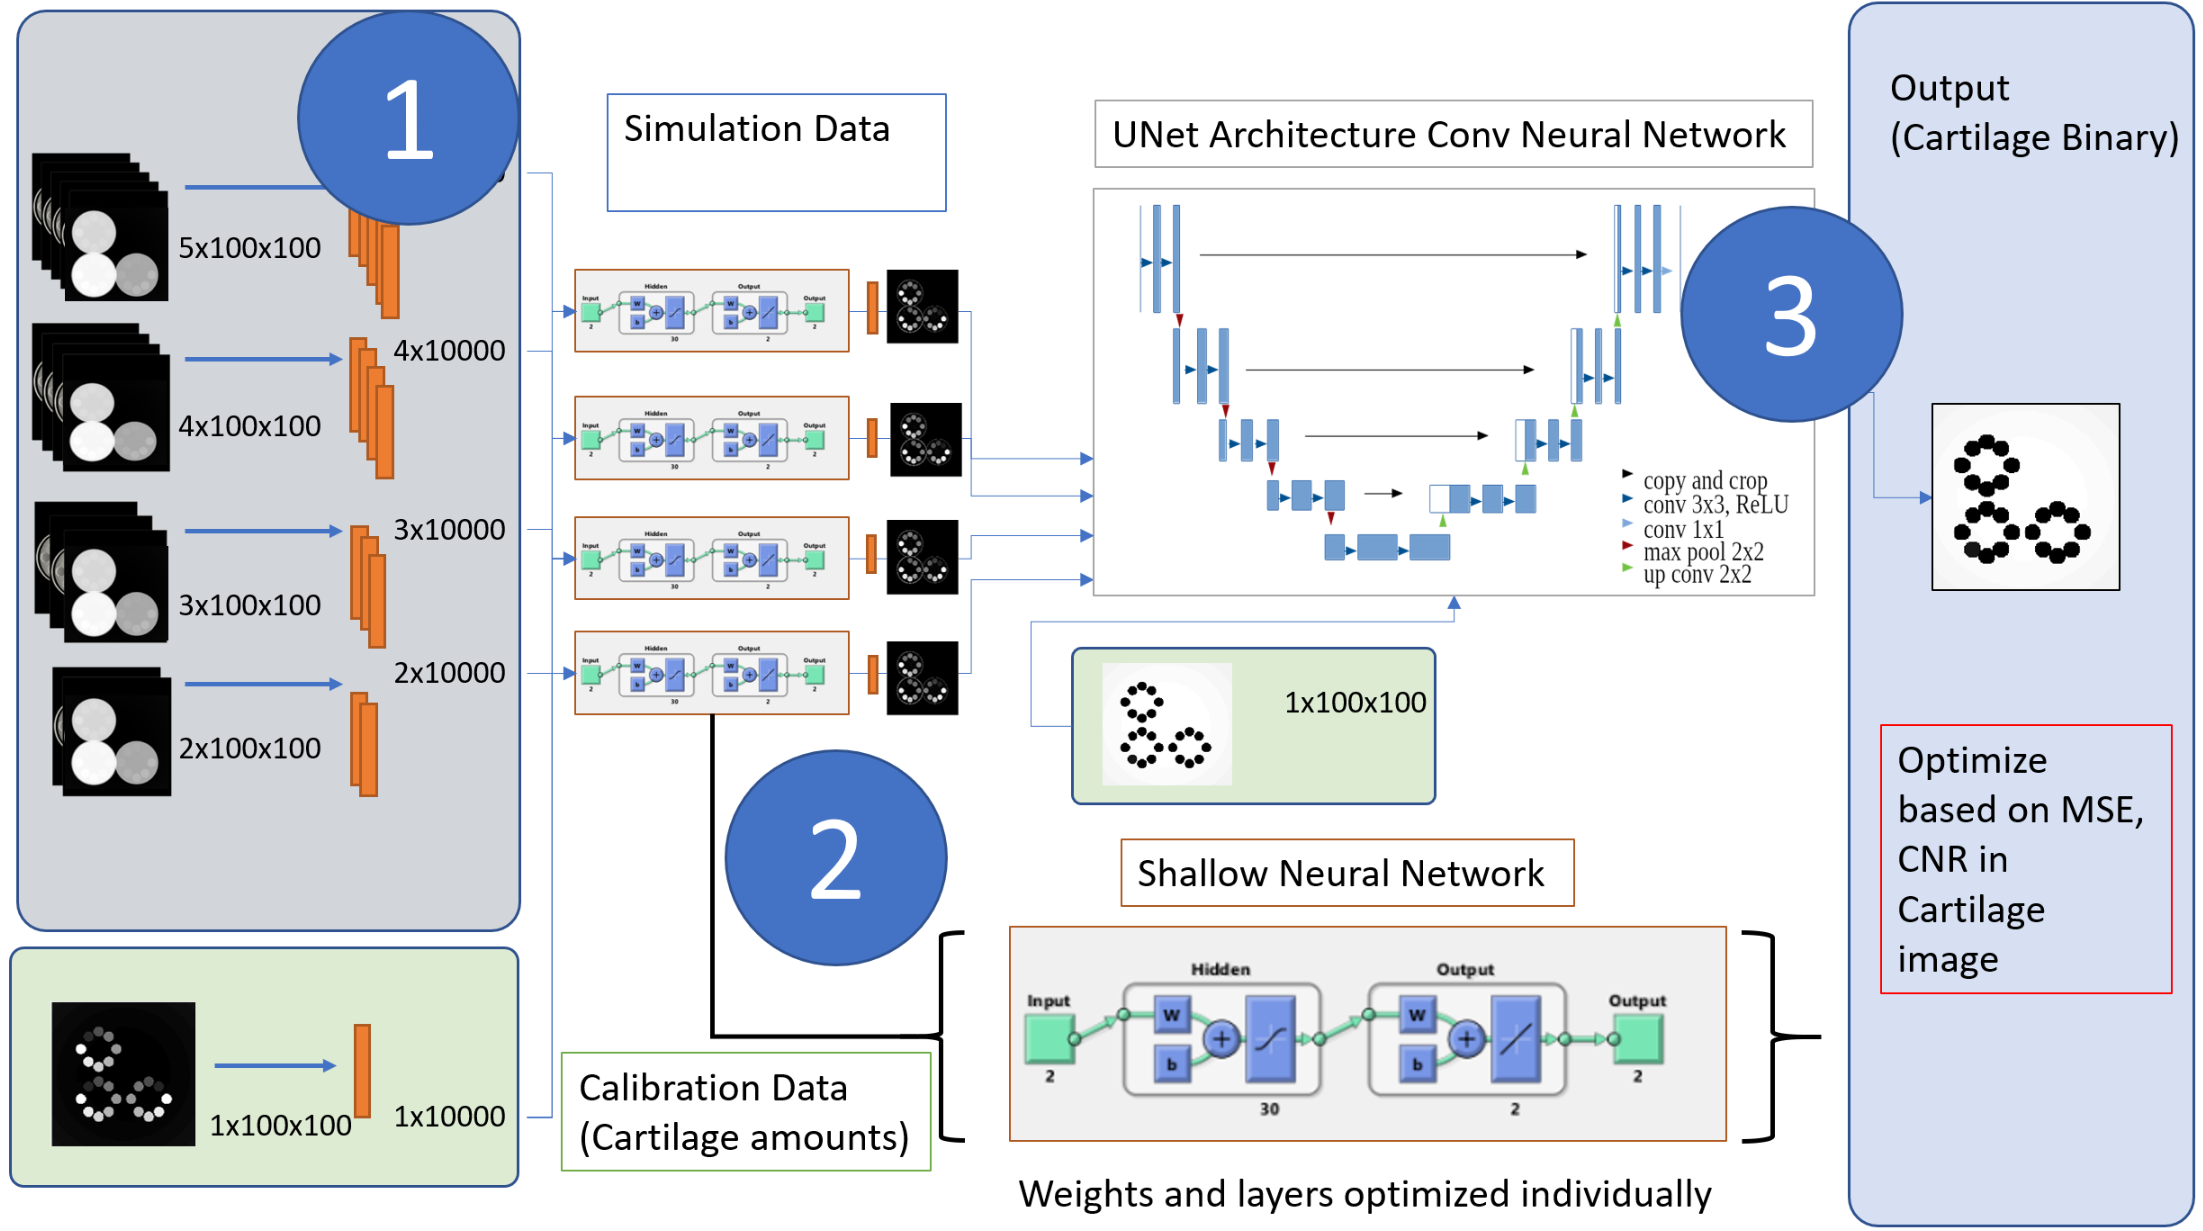
\includegraphics[width=\textwidth]{figures/slide6.png}
\qquad
% "\includegraphics" from the "graphicx" permits to crop (trim+clip)
% and rotate (angle) and image (and much more)
\caption{The complete workflow composed of the three steps: Image simulation, multi-energy subtraction and image segmentation and classification}
\label{fig:i}
\end{figure*}

\begin{equation}
\label{eq:1}
\mu(x,y,E) = a_1(x,y) \frac{1}{E^3}+a_2(x,y) f_{KN}(E)
\end{equation}

Where x, y, and E are the spatial components and energy respectively, $a_1, a_2 $ are the coefficients for the PE and CS component and $f_{KN}(E)$ is the Klein-Nishina function.

In common practice the finding of these coefficients is left to a least squares fitting of the material depth $A_1, A_2$ to the logarithm of image intensity $I_{E_1}, I_{E_2}$ acquired at two energies $E_1$ and $E_2$ to find the parameters ${k_n}, {l_n}$ \cite{Lehmann1981GeneralizedRadiography, Cho2017CalibrationMammography}


\begin{subequations}\label{eq:t}
\begin{align}
\label{eq:t:1}
 \ln(I_{E_1}) = k_1 A_1 + k_2 A_2 +k_3A_1^2 +k_4 A_2^2 +k_5 A_1A_2 
\\
\label{eq:t:2}
\ln(I_{E_2}) = l_1 A_1 + l_2 A_2 +l_3A_1^2 +l_4 A_2^2 +l_5 A_1A_2 
\end{align}
\end{subequations}

This process is not likely to produce the intended parametrization of the intensity of the image as a function of the CS and PE, instead it is more likely to fit to the pixel intensity. To give an example, a least squares fit of depths of bone $(A_1)$ and brain $(A_2)$ to one image will generate fit coefficients that map pixel intensity to bone depth, since one cannot decompose an image into CS and PE in one image. This demonstrates that there is other information for the least squares fit to calibrate on. Given this, it is safe to assume that when given more images the coefficients still have the possibility of fitting based off of the intensity rather than the CS-PE components. Multi-energy images contain more information about the underlying energy dependence of attenuation. Thus we hypothesize that a fitting based on more than two energy bins could better describe the underlying physics processes.

With this idea in mind an n dimensional extension of equation \ref{eq:t} was used in this work where $n$ ranged from 2 to 5:

\begin{subequations}\label{eq:p}
\begin{align}
\label{eq:p:1}
A_1 = \sum_{m=1}^n k_{m} \ln(I_{m})  +\sum_{m=1}^n \sum_{j=1}^n  k'_{j,m} \ln(I_{j}) \ln(I_{m})
\\
\label{eq:p:2}
A_2 = \sum_{m=1}^n l_{m} \ln(I_{m})  +\sum_{m=1}^n \sum_{j=1}^n  l'_{j,m} \ln(I_{j}) \ln(I_{m})
\end{align}
\end{subequations}

\section{Materials and Methods}
\label{sec:methods}

An overview of the total work flow for cartilage segmentation is outlined in figure \ref{fig:i}. The first step consists of image  simulation. The second,  multi-energy subtraction, is  used  to  optimize  the  imaging  parameters. Sitting  on  top  of  this  optimization  is  the  third  step, i.e.  image segmentation  and  classification,  which  demonstrates  the  limitations  of  the  higher  level  feature  classification.  The  code for all  these  steps  can  be  found  in  the  GitHub  repository listed in the Appendix  and  each step is described below in detail.%The code for these steps can be found in the github repository in the Appendix and an overview follows below.
\\

\subsection{Simulation Geometry}

Two imaging geometries were considered in this work: a cone-beam imaging geometry (figure \ref{fig:phantom}) was simulated with an analytical method and parallel-beam geometry was simulated with a Monte Carlo method. Phantoms were imaged with a 60 kVp photon beam, the X-ray source was positioned 30 cm away from the base of the phantom. An idealized PCD was positioned 2 cm behind the phantom.

\subsection{Phantoms}

The phantoms used in this study were composed of solid water (SW) and cartilage (Table 1). The exact composition of the cartilage follows the ICRU-44 \cite{White1989Report44} guidelines and the SW is that of Watanabe 1999 \cite{Watanabe1999DerivationPhotons}. Cartilage was determined to be a good phantom material as cartilage and breast fibrous tissue share similar composition. Animal cartilage is also readily available and durable enough for the construction of an experimental phantom.

\begin{figure}[htbp]
\centering % \begin{center}/\end{center} takes some additional vertical space
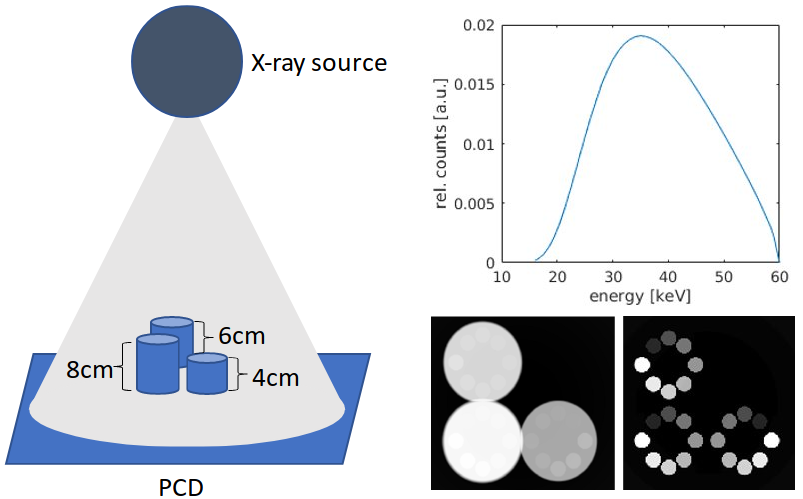
\includegraphics[width=\linewidth]{figures/phantoms4.png}
\qquad
% "\includegraphics" from the "graphicx" permits to crop (trim+clip)
% and rotate (angle) and image (and much more)
\caption{Simulation setup of planar X-ray imaging with PCDs investigated in this work. The spectrum of the X-ray source is shown on the right. A cone-beam X-ray image of the calibration phantoms as well as an image showing the cartilage depths are shown on the bottom right.}
\label{fig:phantom}
\end{figure}

All phantoms were cylindrical in shape. Phantom diameters were 5 cm in the cone-beam simulation and 3.3 cm parallel-beam simulation. Three separate phantoms with SW depths of 8,  6, and 4 cm were modeled in both cases. These depths were chosen to span the range of depths expected in clinical mammography. Inserts of cartilage 0.7 cm in diameter with variable depths were embedded in the phantom's SW body. An image of the three phantoms can be seen in figure \ref{fig:phantom}. Two sets of phantoms, calibration and validation phantoms, were simulated for each imaging geometry.  The calibration phantom contained cartilage inserts of 0 to 4 cm in depth in 0.5 cm increments. The validation phantom contained cartilage inserts of 0.4 cm to 3.9 cm in 0.5 cm increments.

\subsection{X-ray Beam}

Phantoms were imaged with a 60 kVp photon beam generated from a tungsten anode in front of a 0.8 mm beryllium window and 0.1 mm added copper filtration. The spectrum was generated using SpekCalc \cite{Poludniowski2009SpekCalc:Tubes} an analytical X-ray spectrum generator. 

At the detector location, energy bins for all of the simulation were calculated so as to have equal fluence in each energy bin. This was done for optimal statistics as noise increases quadratically with decreasing signal. The cutoff energies for the bins are shown in Table 2.

\begin{table}[]
\label{energies}
\caption{Cutoff energies for energy bins}
\begin{tabular}{ll}
\ Number of energy bins & Cutoff energies {[}keV{]}     \\
2              & 16, 37.5, 60                 \\
3              & 16, 33, 42, 60               \\
4              & 16, 30.8, 37.5, 45, 60       \\
5              & 16, 29.3, 34.8, 40, 46.6, 60
\end{tabular}
\end{table}

\subsection{Analytical Cone-beam Image Generation}

The first image simulation method used Imasim \cite{Landry2013ImaSimRadiology}, a ray tracing application, Gaussian random noise was added to the images to mimic the Poisson statistics of an X-ray imaging system. The detector parameters were made to the specifications of existing CZT PCD (Redlen Technologies, Victoria, BC, Canada) with 0.33 mm pixel pitch.

\subsection{Monte Carlo Parallel-Beam Simulation}

A Monte Carlo simulations to better approximate X-ray interactions with matter, including scatter, were done using Geant4 \cite{Agostinelli2003Geant4Toolkit} extended by TOPAS \cite{Perl2012TOPAS:Applications}. The spectrum was sampled from the same analytical spectrum as used in the cone-beam simulation binned into 0.5-keV bins. The output of each simulation was a $.csv$ file containing energy spectra binned into 0.5-keV steps for each  of the 0.33 mm PCD pixels. The range cutoff for particle transport was 0.05 mm. For each phantom depth 10 trials were performed with different random seed number. Each trial contained $5 \times 10^7$ photons, these trials were summed to make up the images with the different SNR. The detector was considered to be the same as in the analytically-generated images, scoring particles incident on the detector surface. Dose was calculated using the energy deposition. Complete imaging parameter files can be found in the GitHub repository (link shown in the Appendix).

\subsection{Multi-Energy Subtraction Methods}

Image analysis was performed using MATLAB (The Mathworks, Natick, MA). Two different methods were used to extend DES to multi-energy subtraction:

\subsubsection{Least-Squares Fitting}

The image intensities used in the fit for equation \ref{eq:p} were taken from regions of interest (ROIs) covering the circular inserts of the calibration phantom as well as from the body of the phantom and the air surrounding the phantom. The cartilage depth used were the ground truth values from the simulation. The ${k}, {l}$ coefficients in equation \ref{eq:p} were generated from a least squares fit of the cubic equation of log intensities to the depth values. These coefficients were then used to map the validation phantom at every pixel to create a cartilage depth image. This image was compared against the ground truth for validation.

\subsubsection{Non-Linear Fitting}


Equation \ref{eq:p} was fit using a feed forward neural network. With the default set of hyperparameters and used the Levenberg-Marquardt fitting function. The number of hidden layers was optimized individually for each combination of SNR by running 10 trials each for between 5 and 100 layers in 5 layer intervals. The validation data consisted of the cartilage inserts in the validation phantom. The optimal amount of layers was then selected as the result with the lowest mean squared error (MSE) derived from the validation data.

The difference between the linear and non-linear case is the fitting algorithm and in both cases the same data is used from the calibration phantom. In the linear case fitting the data using a least squares method. Conversely, the non-linear case fits the data with a feed-forward neural network. These algorithms are then used to generate cartilage depths from the validation phantom.

The linear and non-linear regression were evaluated by means of CNR and MSE as a function of depth of cartilage and SNR. The CNR and SNR were defined relative to the background consisting of 4 cm of SW. CNR was defined as

\begin{equation}
\label{eq:f}
CNR = \frac{|I^m_{ROI} - I^m_{SW}|}{\sqrt{\sigma^2_{ROI} + \sigma^2_{SW}}}
\end{equation}

Where $I^m$ is the mean intensity. The CNR was bootstrapped to get a 95\% confidence interval.

\begin{figure}[htbp]

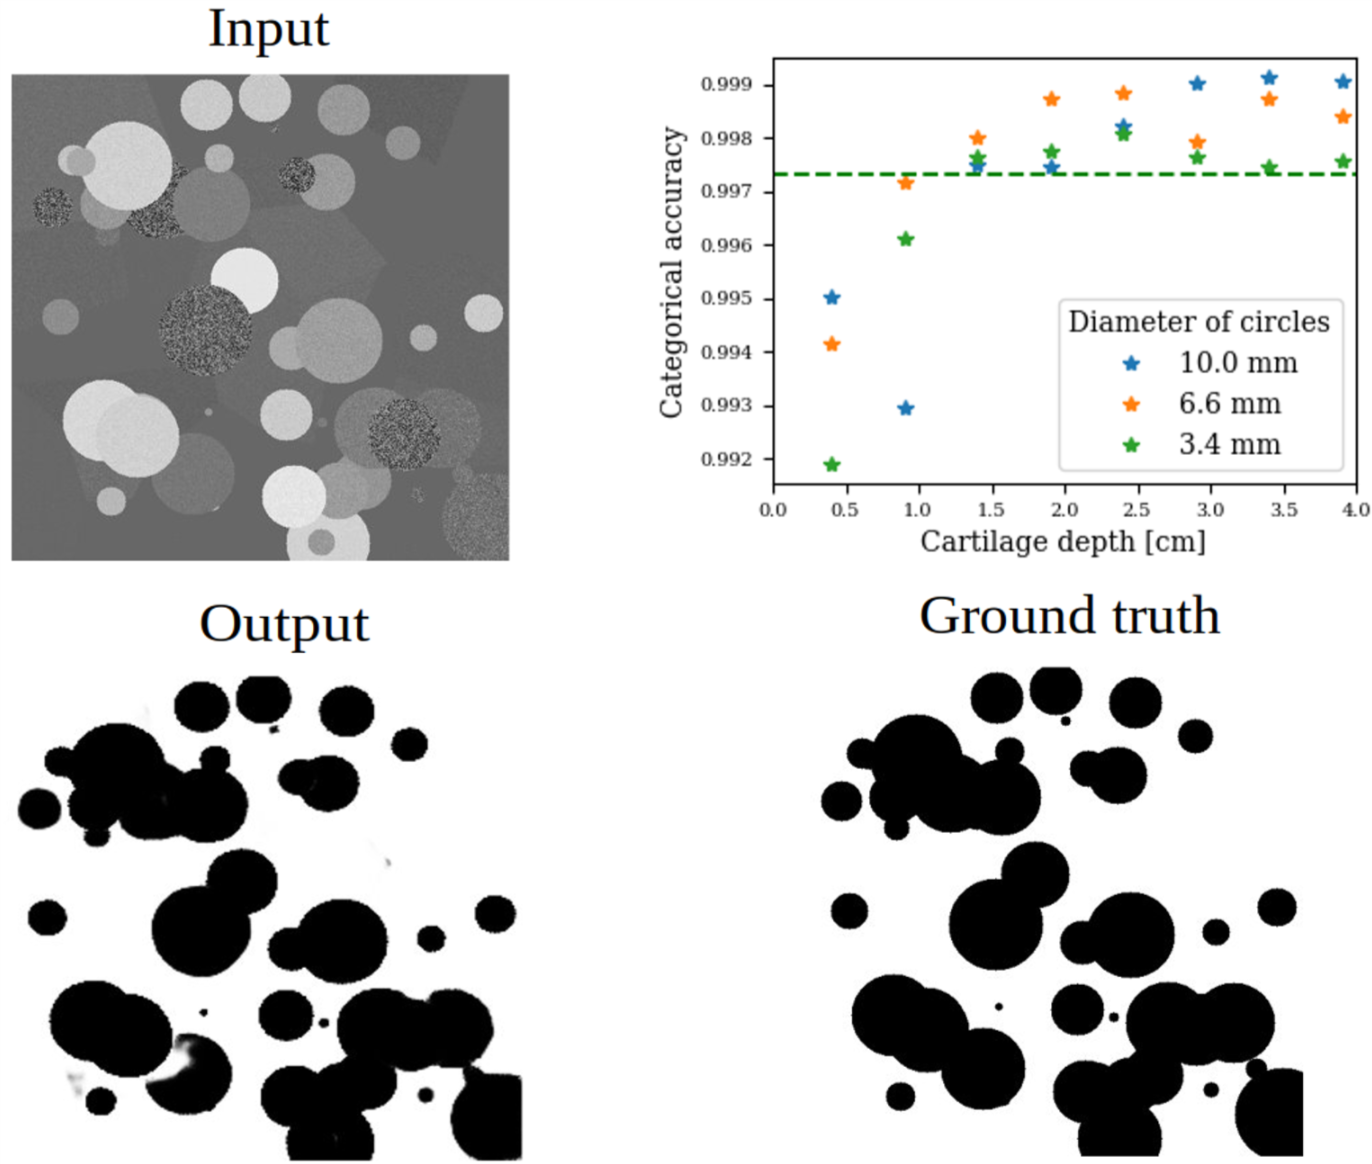
\includegraphics[width=\textwidth]{figures/CNN_1.png}

\caption{The input, ground truth, and output images of for the CNN cartilage segmentation. The regions where the background is similar to the inserts were poorly classified.The top right shows the categorical error for the CNN with respect to cartilage depth and radius of the cartilage objects. The green line is the training accuracy.}
\label{figcali}
\end{figure}

\begin{figure}[htbp]
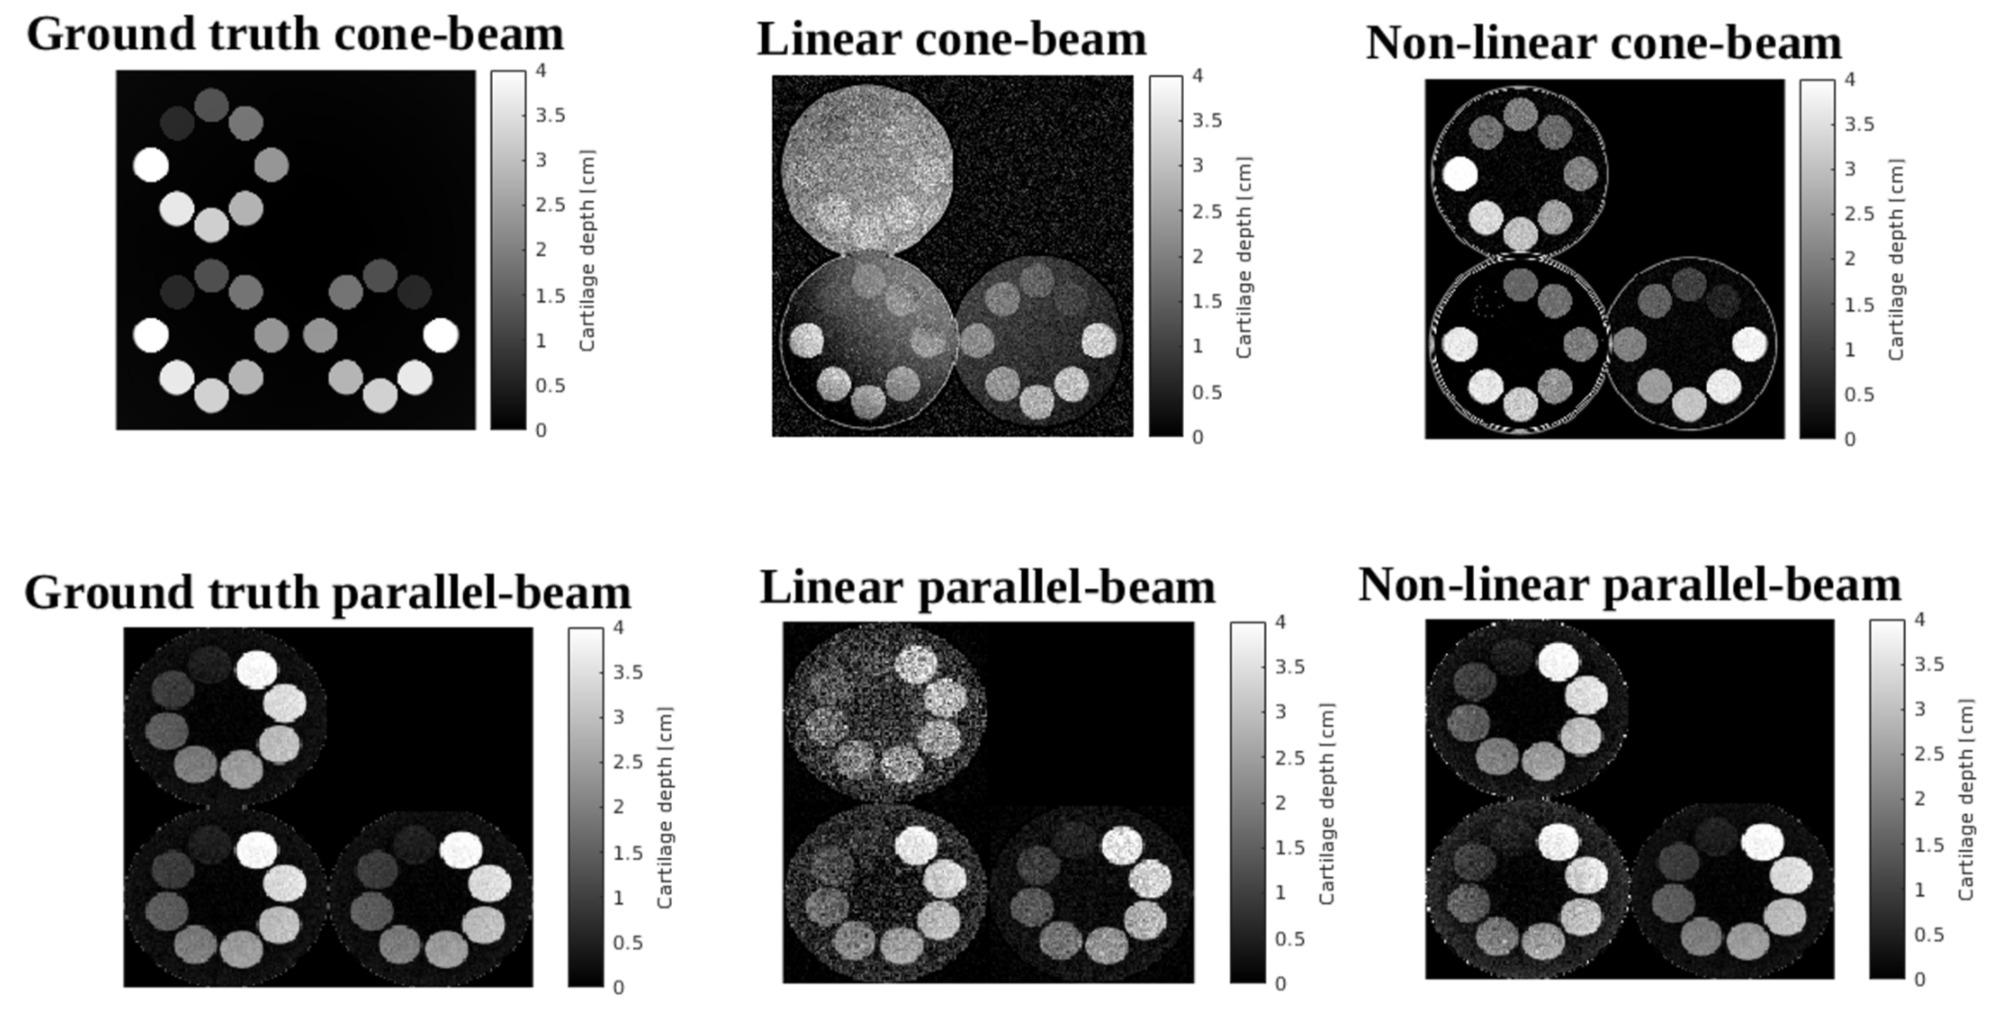
\includegraphics[width=\textwidth]{figures/comparisons_1.png}
\caption{A comparison of the ground truth to the linear and non-linear methods of generating the cartilage depths in the image. The images both contain a 4, 6, and 8 cm phantom on the right, top left, and bottom left respectively. The ground truth for the parallel-beam is actually a simulated image but qualitatively nearly identical to the ground truth.}
\label{figqual}
\qquad
\end{figure}

\subsection{Image Segmentation and Classification}


The input images for the CNN were generated using randomly generated SW polygons as the background. These polygons were assigned image values derived from the cone-beam validation images. Poisson noise was added to each region to achieve a desired SNR of 100. The foreground was composed of circular regions of differing depth of combined SW and cartilage, also derived from the cone-beam calibration data set. Thirty of these simulated images as well as segmented binary images denoting the cartilage were provided to the U-Net for training (figure \ref{figcali}). A data augmentation algorithm was used to generate training samples from the 30 images. The algorithm added small random rotation between 0 and 0.2 rad to the image. Random shifts to the image position between 0 and 0.05 of the image size, as well as shear and zoom to the image, again by a factor of between 0 and 0.05 of the image size. The network was trained with 2000 augmented images per epoch until the verification error remained constant for two consecutive epochs, this amounted to 5 epochs in total. The exact hyperparameters for the network can be found in the accompanying GitHub repository. The network was trained with a NVIDIA P100 Pascal GPU \cite{Lindholm2008NVIDIAArchitecture} with 6 additional CPUs and 32 gigabytes of RAM.

The training data was composed of thirty randomly generated images with the composition mentioned above. The validation was completed on sets of two images created with 100 regions of specific cartilage depth and diameter.  When given the validation data, the trained U-Net output two arrays with values corresponding to each pixel of the image. One array represented the probability of that pixel being cartilage, p(1), and another array representing the probability of it being SW, p(0). The error was investigated using the Keras's categorical error function \cite{Keras-team/keras:Humans}. The categorical error function checks if the output reports p(0) $>$ p(1) for the cartilage regions and the opposite for the SW regions. The error is normalized and linear, thus a value of 1 indicates all points are classified correctly and 0.5 would indicate exactly half the points are classified correctly. 

The training of the U-Net can be accessed through a cyberhub environment \cite{Herwig2018Cyberhubs:Astronomy} on an internet browser using the link in the Appendix.

\section{Results}

% \begin{figure*}[htbp]



% 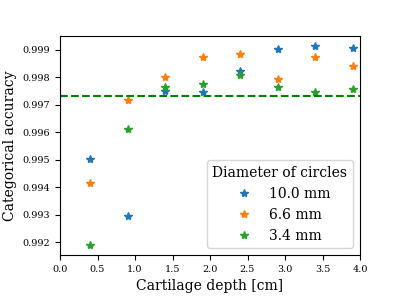
\includegraphics[width=\textwidth]{figures/unet_acc.png}
% \caption{Categorical error for the CNN with respect to cartilage depth and radius of the cartilage objects. The green line is the training accuracy.}
% \label{figp}
% \end{figure*}

\subsection{Multi-energy Subtraction Results}

\begin{figure*}[htbp]
    \centering
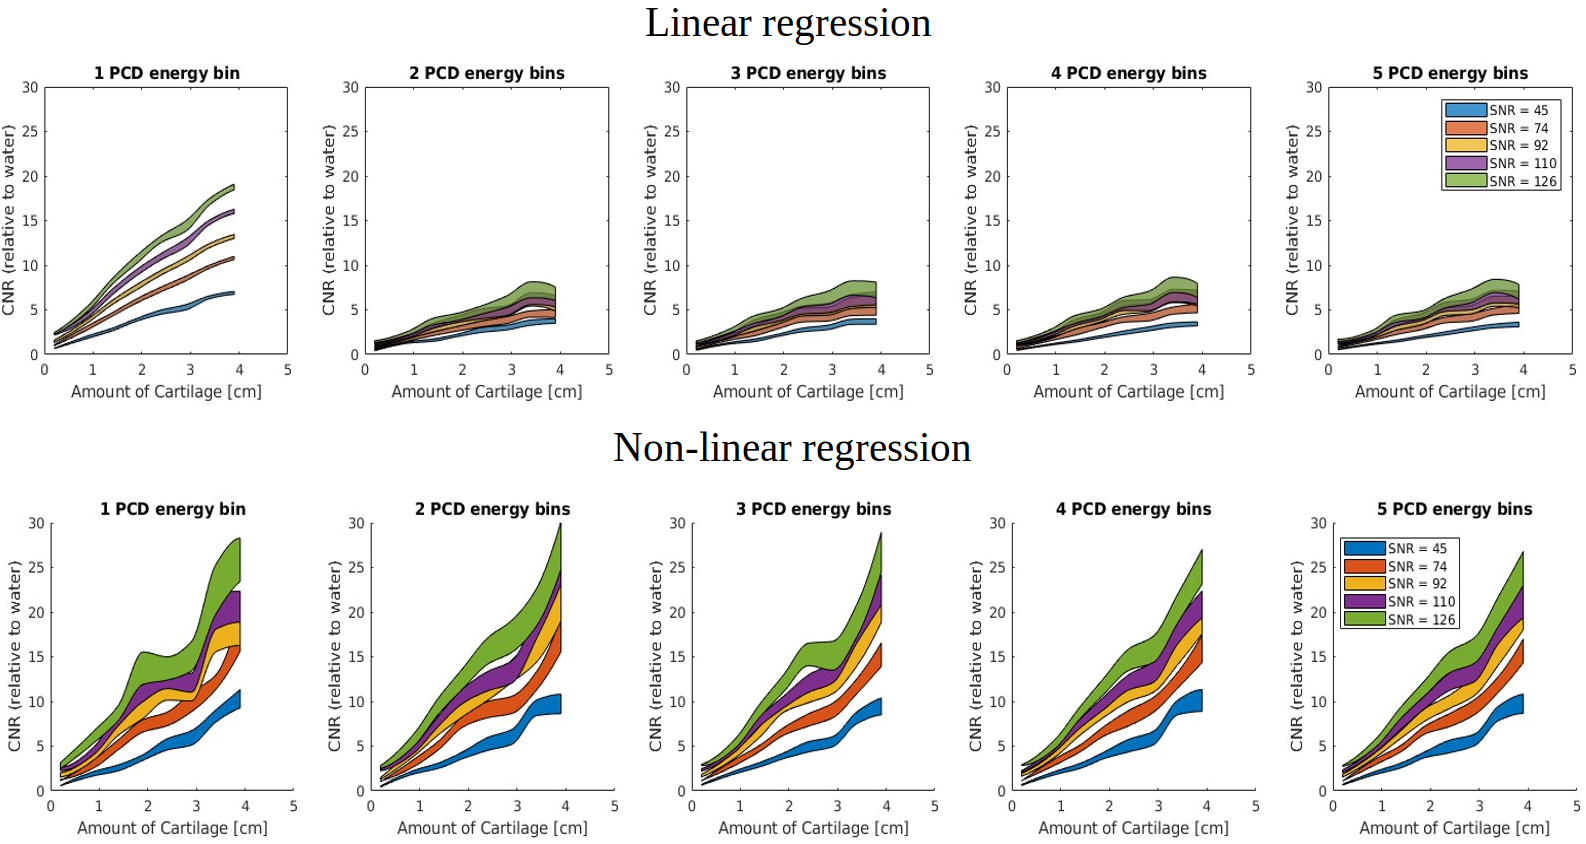
\includegraphics[width = \textwidth,trim={10.5cm 0cm 0cm 0cm},clip]{figures/CNR_pb.png}
    \caption{CNR for the parallel-beam Monte Carlo simulations for the linear mapping (top) and the non-linear mapping (bottom) as a function of the number of PCD energy bins. All values are bootstrapped to find the 95 percent confidence interval. The non-linear results are above 4 indicating adequate CNR for human identification of structures.}
    \label{fig:CNR}
\end{figure*}

Figure \ref{figqual} shows outputs of the linear and non-linear regressions applied to the cone-beam and pencil-beam images. The CNR as a function of number of PCD energy bins, cartilage depth and image SNR for both the linear and non-linear energy subtraction methods is shown in figure \ref{fig:CNR}. The CNR proved to be similar for the images in question. Based on figure \ref{fig:CNR} and Rose criterion \cite{Rose1975Vision:Electronic}, the minimum detectable depth was very similar for the non-linear multi-energy regression. In the linear regression all energy bins had similar CNRs, but was lower than the equivalent non-linear regression image. Since it was equivalent throughout the non-linear images CNR was not used as the deciding factor in image segmentation optimization.

Results from multi-energy subtraction can be seen in figure \ref{fig:err}. The non-linear regression was seen to have higher CNR  in the majority of cases and lower MSE in all cases compared to the linear regression. The lowest MSE of cartilage depth calculation for both the cone-beam and the parallel-beam image generation was found for four energy bins over all SNR. Four energy bins was therefore deemed the optimal number of energy bins given our imaging setup. Figure \ref{figqual} error in the linear regression came from failure to differentiate between the cartilage and SW in the 6 cm phantom.

The Monte Carlo results from the parallel-beam imaging agree closely with the analytical cone beam results in the non-linear case as seen on the right of figure \ref{fig:err}. However, in the linear case there is variation between the two surfaces, with the cone-beam geometry over-fitting for the high SNR at low energy. It was seen that for high enough SNR the non-linear regression could nearly fully map to the depth of cartilage with very low error $<$ 0.05 cm. Overall, the minimum of the error was at 4 energy bins for all of the SNR in both the cone-beam and the parallel-beam geometries. The MSE with 4 energy bins compared to 2 energy bin was reduced by 19\% and 4\% for the cone-beam and parallel-beam cases, respectively.

\begin{figure*}[htbp]
    \centering
\adjincludegraphics[width = \textwidth,trim={4cm 8cm 4cm 8cm},clip]{figures/Error_Comparison_tnr.png}
    \caption{Cartilage estimation MSE for the cone-beam (left) and the parallel-beam (middle) geometries, and a comparison of the parallel and cone-beam errors for the superior non-linear regression method (right).}
    \label{fig:err}
\end{figure*}

\subsection{Segmentation and Classification Results}

Results from the segmentation and classification in terms of MSE of cartilage depth are presented in figure \ref{figcali} and figure \ref{fig:err}. The accuracy of the training (0.9973 after 4 epochs) was seen to generalize very well to the test set with all accuracies above 0.99 when tested on images of different sizes and cartilage depths. Figure \ref{fig:err} shows that the accuracy is reduced for smaller sizes and lower cartilage depths but is still very good for all values tested. The accuracy quoted above is measuring the pixel by pixel error, however arguably more important than the pixel by pixel classification is whether the larger circular regions can be segmented from the SW background.  Looking at classification on a region by region basis in the lowest cartilage depth image analysis showed that all cartilage regions could be identified. This was done by manually counting the cartilage regions in the ground truth and the output image.

\section{Discussion and Conclusions}

The accuracy of automated cartilage tissue segmentation for planar X-ray imaging with a PCD was investigated. Across all studied SNRs, four energy bins resulted in the lowest MSE in cartilage depth calculation for both investigated imaging geometries 
figure \ref{fig:err} Compared to the dual-energy case, the MSE was 19\% and 4\% lower for the cone-beam and parallel-beam cases, respectively. This implies that there are potential gains in soft tissue segmentation when using a PCD with more than two energy bins. Likewise, a non-linear regression method should be used instead of a least squares fit as this resulted in lower MSE in all cases. Overall, four energy bins and the non-linear method would result in the highest accuracy in lesion detection for a given imaging dose.

In all image generation SNR was used as an independent variable. Ideally one would use dose instead of SNR since we would like to find the minimal imaging dose for accurate tissue segmentation. This change of variable was done since we did not have an accurate metric for dose in our analytic simulation. Thus to have a consistent independent variable between simulations SNR was used as a proxy for dose in both the analytical and Monte Carlo simulations. This is allowable since imaging dose increases with increasing SNR.

The reduction in MSE for cartilage depth calculation was SNR dependent with the largest changes in MSE at SNR of 50-100 in the cone-beam case. The average MSE was reduced 29\% in this region compared to the two energy bin case. This shows potential for this method to be used in low dose imaging. However, in the parallel-beam Monte Carlo simulation, which included scatter, the error was relatively constant over all SNR. Thus an optimal X-ray imaging method with PCDs should include scatter reduction techniques or should be performed with a fan-beam geometry to limit scatter. It is expected that the simulation results are dependent on the imaging beam energy. Note that in this work we used a 60 kVp beam with a 0.8 mm beryllium window and 0.1 mm added copper filtration. For imaging of thicker object, a higher energy beam would be more appropriate and should be investigated for spectral projection imaging.

The results from the multi-energy subtraction method were not dependent on the beam geometry as the methods had similar error in both cone-beam and parallel-beam geometries (figure \ref{fig:err}). The MSE was slightly lower for the cone-beam. This was expected as the cone-beam method was idealized and did not include X-ray scatter that deteriorates image quality and affects image subtraction. The classification step had accurate results using the output of the neural network non-linear regression at an SNR of 100; all cartilage depths resulted in a categorical accuracy of greater than 0.99 (figure \ref{figcali} top right). 

A consideration in the work was to make the segmentation method easy to adapt to experimental data. To do this one would need a two material calibration phantom to calibrate the non-linear regression and 30 segmented images of lesions to train the CNN. Since manual segmentation is superior to that of the CNN for diagnostics \cite{Ronneberger2015U-Net:Segmentation}, removing the U-Net layer and manually segmenting the output image of the non-linear regression would produce optimal results. Likewise, the U-Net could be included but used as second opinion to compare to the manual segmentation.

Cartilage was used as a phantom material in this study as animal cartilage is readily available and durable enough to be machined to precise depths. Another set of materials that are not as readily available but have clinical significance are fibrous and adipose tissue. Breast density, as described by the amount of fibrous tissue in the breast is a risk factor for breast cancer \cite{McCormack2006BreastMeta-analysis}. Further simulation work could quantify the material dependence of  dual- and multi-energy subtraction methods by comparing results from a fibrous-adipose tissue phantom to the presented SW-cartilage phantom. 

Further work should also incorporate simulations of the response of the spectral detectors in terms of energy deposition, as well as other factors in spectral detectors, such as charge sharing, small pixel effects and other effects that reduce the accuracy of the detector. Overall, the primary focus of further work will be the validation of this method using experimental PCD images.



 \section*{Acknowledgments}

The authors would like to thank Chelsea Dunning for her contribution to the TOPAS code and to Joseph Perl for helping us in obtaining a TOPAS licence. Additional thanks goes to Compute Canada for access to their research computing resources. This work was funded in part by an NSERC Engage and NSERC Discovery Grant, as well as the Canada Research Chair program. 



% or
\appendix{}
\section{Git Repository}
The GitHub repository with all code necessary to reproduce data presented in this paper can be found at \href{https://github.com/jerichooconnell/unet}{https://github.com/jerichooconnell/unet}. To explore the neural network training a binder link has been set up at \href{https://mybinder.org/v2/gh/jerichooconnell/unet/master?filepath=unet\%2FtrainUnet.ipynb}{goo.gl/yXRnfM}.





\bibliographystyle{JHEP}
\bibliography{references}


\vfill

% Can be used to pull up biographies so that the bottom of the last one
% is flush with the other column.
%\enlargethispage{-5in}



% that's all folks
\end{document}
% \title{Journal of Instrumentation (JINST) template}


% %% %simple case: 2 authors, same institution
% %% \author{A. Uthor}
% %% \author{and A. Nother Author}
% %% \affiliation{Institution,\\Address, Country}

% % more complex case: 4 authors, 3 institutions, 2 footnotes
% \author[a,b,1]{F. Irst,\note{Corresponding author.}}
% \author[c]{S. Econd,}
% \author[a,2]{T. Hird\note{Also at Some University.}}
% \author[c,2]{and Fourth}

% % The "\note" macro will give a warning: "Ignoring empty anchor..."
% % you can safely ignore it.

% \affiliation[a]{One University,\\some-street, Country}
% \affiliation[b]{Another University,\\different-address, Country}
% \affiliation[c]{A School for Advanced Studies,\\some-location, Country}

% % e-mail addresses: only for the corresponding author
% \emailAdd{first@one.univ}



% \abstract{Abstract...}



% \keywords{Only keywords from JINST's keywords list please}


% \arxivnumber{1234.56789} % only if you have one


% % \collaboration{\includegraphics[height=17mm]{example-image}\\[6pt]
% %   XXX collaboration}
% % or
% \collaboration[c]{on behalf of XXX collaboration}


% % if you write for a special issue this may be useful





% \begin{document}
% \maketitle
% \flushbottom

% \section{Introduction}
% \label{sec:intro}

% The modern production line seeks efficiency through automation of human roles. When used properly, automation can increase production and lower cost. With automation, however, comes an increased pressure on quality control: Machines, unlike humans, are not expected to know if the product is contaminated by their actions. The ideal quality control in these situations is what is known as nondestructive testing (NDT), testing that leaves the product unchanged. The ideal NDT method is the use of XRay imaging. Current XRay imaging capabilities are limited to the detection of large differences in material density. However, new photon count detectors (PCDs) allow for XRay imaging to be extended to materials of similar composition. This application is particularly important in the meat processing industry where cartilage and tissue share similar compositions.

% In this work, spectral imaging is examined for the detection of cartilage in soft tissue. This is meant to be a direct application to the poultry industry. However, these results apply equally to the planar XRay discrimination of other materials with two components of similar composition. Other works have been done to investigate dual energy imaging in this application (???), but the extension to more energies has not been seen.

% It is important to note some other considerations in this problem: Firstly, this system must image objects on a conveyor belt moving at 0.5 m/s. And secondly to be cost effective the xray tube should be one with low current. Thus when discussing this problem it is essential to look at xray imaging for a photon starved system. 

% This work aims to examine exactly what the minimal imaging parameters are for systems to be accurate. Specifically, to examine the detection of different thicknesses of contaminant under different xray exposures. To this aim, the independent variables in question will be signal to noise ratio (SNR) and thickness of cartilage in cm.

% The novelty of this work is twofold: The first novel component is the modeling of a REDLEN cadmium zinc telluride semiconductor PCD. Secondly, the cartilage identification method is novel in that it extends dual energy extraction of (???) to many energies. This method is coupled with a convolutional neural network (CNN) , the architecture being the U-Net achitecture which is shown to be optimal for segmentation. Overall, this work aims to examine the application of CNNs and photon counting detectors (PCDs) in nondestructive imaging.

% \section{Methods}
% \label{sec:methods}

% An overview of the total work flow can be seen in figure~\ref{fig:i}:


% \begin{figure}[htbp]
% \centering % \begin{center}/\end{center} takes some additional vertical space
% \includegraphics[width=\textwidth]{figures/Slide4.jpg}
% \qquad
% % "\includegraphics" from the "graphicx" permits to crop (trim+clip)
% % and rotate (angle) and image (and much more)
% \caption{\label{fig:i} Complete work flow U-Net image reproduced with permission (???) from ....}
% \end{figure}

% Steps 1 (Image Simulation) and 2 (Multi-Energy Subtraction) are used to optimize the imaging parameters while the third step (Image Segmentation and Classification) is used to determine the limitations of the higher level classification.

% \subsection{Image Simulation}
% \subsubsection{Phantoms, Spectra and General Parameters}

% The phantoms used in this study were composed of Cartilage and Solid Water, the exact composition of the cartilage follows the ICRU-44 guidelines and the water is that of Watanabe 1999. 

% Table(*???)

% Three seperate phantoms were modeled of three diferent water thickness 8,  6, and 4 cm respectively. These thicknesses were chosen to span the range of thicknesses expected in the calibration, smaller phantoms were investigated but resulted in less failure of differentiation. In this phantom smaller inserts of 0:4 cm in 0.5cm increments were embedded, it is noted that the best interpolation would be the use of the Chebyshev nodes for this range as proposed by (???) however it has also been demonstrated that machinists prefer lengths that are rational numbers.

% \begin{figure}[htbp]
% \centering % \begin{center}/\end{center} takes some additional vertical space
% 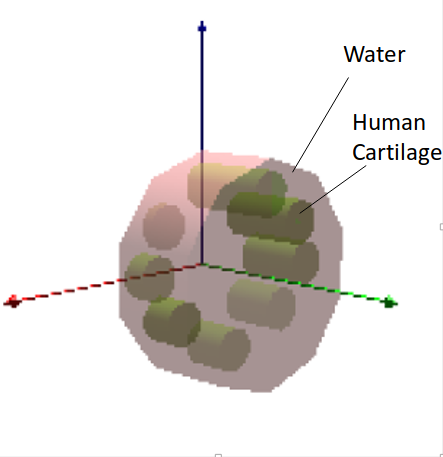
\includegraphics[width=0.4\textwidth]{figures/phantom.png}
% \qquad
% 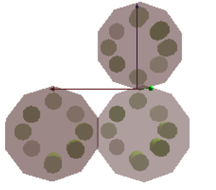
\includegraphics[width=.4\textwidth,]{figures/phantom3.png}
% % "\includegraphics" from the "graphicx" permits to crop (trim+clip)
% % and rotate (angle) and image (and much more)
% % "\includegraphics" from the "graphicx" permits to crop (trim+clip)
% % and rotate (angle) and image (and much more)
% \caption{\label{fig:i}  An image of one of the phantoms and all three}
% \end{figure}

% A similar phantom was used for the validation step save but with inserts of 0.4:3.9 cm in 0.5 cm increments.

% The spectra used was a simple 60 kVp spectrum with generated from a tungsten anode with 0.8 mm beryllium, 30 cm air and 0.1 mm copper filtration. The detector was an ideal integrating detector over the energy range indicated 

% A note should be made on the binning of the energies, energy bins for all of the simulation were calculated so as to have equal fluency in the each energy bin. These bins were calculated by integrating over the desired fraction of the spectra. This was done for optimal statistics as noise increases quadratically with decreasing signal equal fluence results in the best average signal to noise in the images. 

% \subsubsection{Analytical}

% Two separate types of simulations were preformed in this work, the first image simulation method uses Imasim (???) a ray tracing application that provides perfect ray tracings, Gaussian random noise was added to the images to mimic the Poisson statistics that occur in a normal image, the imaging parameters were made to the specifications of the REDLEN detector :

% table()

% \subsubsection{Monte Carlo}

% A monte carlo simulation was done using Geant4 extended by TOPAS, the spectrum was sampled from a analytically simulating with 89 points sampled over the spectra. For each phantom thickness 10 trials were preformed with different random number seeds with 5000000 photons each, these trails were summed to make up the images with the different signals. Complete imaging parameter files can be found in the github repository.


% \subsection{Multi-Energy Subtraction}


% Alvarez et al. mention many times in various papers that there is no improvement to dual energy subtraction when using more energies. This stems from the fact that the photoelectric component and the compton scattering component of the photon interactions fully describe the system, therefore two components can span this space and further images will just give linearly dependant information. In less words;



% \begin{equation}
% \label{eq:1}
% \mu(x,y,E) = a_1(x,y) \frac{1}{E^3}+a_2(x,y) f_{KN}(E)
% \end{equation}

% Where x, y and E need no explanation $\mu$ is the attenuation and $a_1, a_2 $ are coefficients for the photoelectric effect and Compton scattering component and $f_{KN}(E)$ is the Klein-Nishina function.

% However the finding of these coefficients is generally left to a least squares fitting of the material thicknesses $A_1, A_2$ to the log intensity $I_{energy 1}, I_{energy 2}$ of the image to find the parameters ${k_n}, {l_n}$ (ref ref ref???)


% \begin{subequations}\label{eq:t}
% \begin{align}
% \label{eq:t:1}
%  \ln(I_{energy 1}) = k_1 A_1 + k_2 A_2 +k_3A_1^2 +k_4 A_2^2 +k_5 A_1A_2 
% \\
% \label{eq:t:2}
% \ln(I_{energy 2}) = l_1 A_1 + l_2 A_2 +l_3A_1^2 +l_4 A_2^2 +l_5 A_1A_2 
% \end{align}
% \end{subequations}

% However this practise is not likely to produce the intended parametrization of the intensity of the image as a function of the Compton scattering and Photoelectric effect, instead is mush more likely to fit to the pixel intensity. To give an example, a least squares fit of thickness of bone $(A_1)$ and brain $(A_2)$ to one image will generate fit coefficients that map pixel intensity to bone thickness, since one cannot parametrize decompose an image into compton scattering and photoelectric effect in one image. This demonstrates that there is other information for the least squares fit to calibrate on. Given this it is safe to assume that when given more images the coefficients still have the possibility of fitting based off of the intensity rather than the CS/PE. Since the fit is not based entirely off of CS/PE it is possible that more images will give a better fit that will be based more on the CS/PE components in the material and less on the raw pixel intensity.

% Thus the idea of more energies being unececessary was put on hold and \ref{eq:y} was bravely extended to n energies as

% \begin{subequations}\label{eq:p}
% \begin{align}
% \label{eq:p:1}
% A_1 = \sum_{m=1}^n k_{m} \ln(I_{m})  +\sum_{j=1}^n  k'_{j,m} \ln(I_{j}) \ln(I_{m})
% \\
% \label{eq:p:2}
% A_2 = \sum_{m=1}^n l_{m} \ln(I_{m})  +\sum_{j=1}^n  l'_{j,m} \ln(I_{j}) \ln(I_{m})
% \end{align}
% \end{subequations}


% \subsubsection{Least-Squares Fitting}

% The least squares regression used was similar to what is described in \ref{eq:p} extended to n energies
% the intensities used in the fit were taken from the circular inserts of the phantom.

% \subsubsection{Non-Linear Fitting}

% The same equation \ref{eq:p} was fit using a feed forward neural network (MATLAB feedforwardnet(???)), the hyper parameters used were the defaults save the number of hidden layers was optimized individually for each combination of SNR by running 10 trials each for 5 to 100 layers in 5 layer interval, the optimal amount of layers was then selected as the result with the lowest mean squared error MSE on the validation data.

% \subsection{Image Segmentation and Classification}

% The input for the CNN is generated randomly assigned polygons as the background, these polygons are assigned image values taken from the validation images in Imasim with Poisson noise added to get the desired signal to noise ratio. The background polygons are composed of water in this way. The foreground is composed of circular regions of differing thicknesses of combined water and cartilage again taken from the Imasim validation data set, the U-Net is also provided a segmentation for training as seen in figure \ref{fig:j}. The exact hyperparameters for the network can be found at github (???).


% \begin{figure}[htbp]
% \centering % \begin{center}/\end{center} takes some additional vertical space
% 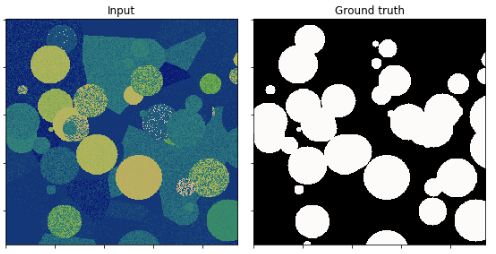
\includegraphics[width=\textwidth]{figures/CNN_val.png}
% \qquad
% % "\includegraphics" from the "graphicx" permits to crop (trim+clip)
% % and rotate (angle) and image (and much more)
% \caption{\label{fig:j} Complete work flow U-Net image reproduced with permission (???) from ....}
% \end{figure}

% \section{Results}

% The linear and non-linear regression were evaluated by means of CNR, MSE as a function of amount cartilage ($T_c$) and SNR. With the CNR and SNR defined relative to 4cm of water, specifically

% \begin{equation}
% \label{eq:f}
% CNR = \frac{|I^m_{ROI} - I^m_{H_2O}|}{\sqrt{\sigma^2_{ROI} + \sigma^2_{H_2O}}}
% \end{equation}
% The CNR was bootstrapped to the 95\% confidence interval which is shown as a band in figure \ref{}

% If you want some equations without the tag (number), please use the available
% starred-environments. For example:
% \begin{equation*}
% x = 1
% \end{equation*}

% The amsmath package has many features. For example, you can use use
% \texttt{subequations} environment:
% \begin{subequations}\label{eq:y}
% \begin{align}
% \label{eq:y:1}
% a & = 1 
% \\
% \label{eq:y:2}
% b & = 2
% \end{align}
% and it will continue to operate across the text also.
% \begin{equation}
% \label{eq:y:3}
% c = 3
% \end{equation}
% \end{subequations}
% The references will work as you'd expect: \eqref{eq:y:1},
% \eqref{eq:y:2} and \eqref{eq:y:3} are all part of \eqref{eq:y}.

% A similar solution is available for figures via the \texttt{subfigure}
% package (not loaded by default and not shown here).
% All figures and tables should be referenced in the text and should be
% placed on the page where they are first cited or in
% subsequent pages. Positioning them in the source file
% after the paragraph where you first reference them usually yield good
% results. See figure~\ref{fig:i} and table~\ref{tab:i}.

% \begin{figure}[htbp]
% \centering % \begin{center}/\end{center} takes some additional vertical space
% \includegraphics[width=.4\textwidth,trim=30 110 0 0,clip]{example-image-a}
% \qquad
% \includegraphics[width=.4\textwidth,origin=c,angle=180]{example-image-b}
% % "\includegraphics" from the "graphicx" permits to crop (trim+clip)
% % and rotate (angle) and image (and much more)
% \caption{\label{fig:i} Always give a caption.}
% \end{figure}


% \begin{table}[htbp]
% \centering
% \caption{\label{tab:i} We prefer to have borders around the tables.}
% \smallskip
% \begin{tabular}{|lr|c|}
% \hline
% x&y&x and y\\
% \hline
% a & b & a and b\\
% 1 & 2 & 1 and 2\\
% $\alpha$ & $\beta$ & $\alpha$ and $\beta$\\
% \hline
% \end{tabular}
% \end{table}

% We discourage the use of inline figures (wrapfigure), as they may be
% difficult to position if the page layout changes.

% We suggest not to abbreviate: ``section'', ``appendix'', ``figure''
% and ``table'', but ``eq.'' and ``ref.'' are welcome. Also, please do
% not use \texttt{\textbackslash emph} or \texttt{\textbackslash it} for
% latin abbreviaitons: i.e., et al., e.g., vs., etc.



% \section{Sections}
% \subsection{And subsequent}
% \subsubsection{Sub-sections}
% \paragraph{Up to paragraphs.} We find that having more levels usually
% reduces the clarity of the article. Also, we strongly discourage the
% use of non-numbered sections (e.g.~\texttt{\textbackslash
%   subsubsection*}).  Please also see the use of
% ``\texttt{\textbackslash texorpdfstring\{\}\{\}}'' to avoid warnings
% from the hyperref package when you have math in the section titles



% \appendix
% \section{Some title}
% Please always give a title also for appendices.





% \acknowledgments

% This is the most common positions for acknowledgments. A macro is
% available to maintain the same layout and spelling of the heading.

% \paragraph{Note added.} This is also a good position for notes added
% after the paper has been written.





% % We suggest to always provide author, title and journal data:
% % in short all the informations that clearly identify a document.

% \begin{thebibliography}{99}

% \bibitem{a}
% Author, \emph{Title}, \emph{J. Abbrev.} {\bf vol} (year) pg.

% \bibitem{b}
% Author, \emph{Title},
% arxiv:1234.5678.

% \bibitem{c}
% Author, \emph{Title},
% Publisher (year).


% % Please avoid comments such as "For a review'', "For some examples",
% % "and references therein" or move them in the text. In general,
% % please leave only references in the bibliography and move all
% % accessory text in footnotes.

% % Also, please have only one work for each \bibitem.


% \end{thebibliography}
% \end{document}
